\documentclass[12pt]{article}
%\usepackage{natbib}
\usepackage{blindtext}
\usepackage[utf8]{inputenc}
\usepackage{graphicx}
\usepackage{url}
\usepackage{float}

\usepackage{listings} % Required for inserting code snippets
\usepackage[usenames,dvipsnames]{color} % Required for specifying custom colors and referring to colors by name

\definecolor{DarkGreen}{rgb}{0.0,0.4,0.0} % Comment color
\definecolor{highlight}{RGB}{255,251,204} % Code highlight color

\lstdefinestyle{Style1}{ % Define a style for your code snippet, multiple definitions can be made if, for example, you wish to insert multiple code snippets using different programming languages into one document
language=Perl, % Detects keywords, comments, strings, functions, etc for the language specified
backgroundcolor=\color{highlight}, % Set the background color for the snippet - useful for highlighting
basicstyle=\footnotesize\ttfamily, % The default font size and style of the code
breakatwhitespace=false, % If true, only allows line breaks at white space
breaklines=true, % Automatic line breaking (prevents code from protruding outside the box)
captionpos=b, % Sets the caption position: b for bottom; t for top
commentstyle=\usefont{T1}{pcr}{m}{sl}\color{DarkGreen}, % Style of comments within the code - dark green courier font
deletekeywords={}, % If you want to delete any keywords from the current language separate them by commas
%escapeinside={\%}, % This allows you to escape to LaTeX using the character in the bracket
firstnumber=1, % Line numbers begin at line 1
frame=single, % Frame around the code box, value can be: none, leftline, topline, bottomline, lines, single, shadowbox
frameround=tttt, % Rounds the corners of the frame for the top left, top right, bottom left and bottom right positions
keywordstyle=\color{Blue}\bf, % Functions are bold and blue
morekeywords={}, % Add any functions no included by default here separated by commas
numbers=left, % Location of line numbers, can take the values of: none, left, right
numbersep=10pt, % Distance of line numbers from the code box
numberstyle=\tiny\color{Gray}, % Style used for line numbers
rulecolor=\color{black}, % Frame border color
showstringspaces=false, % Don't put marks in string spaces
showtabs=false, % Display tabs in the code as lines
stepnumber=5, % The step distance between line numbers, i.e. how often will lines be numbered
stringstyle=\color{Purple}, % Strings are purple
tabsize=2, % Number of spaces per tab in the code
}

% Create a command to cleanly insert a snippet with the style above anywhere in the document
\newcommand{\insertcode}[2]{\begin{itemize}\item[]\lstinputlisting[caption=#2,label=#1,style=Style1]{#1}\end{itemize}} % The first argument is the script location/filename and the second is a caption for the listing



\begin{document}

\title{Methods for classification of handwritten written digits}
\date{\today}
\author{Kris Kiradjiev and Mel Beckerleg}
\maketitle

\section{Overview}

Image recognition is an important technique in a range of fields, from security and surveillance, to intelligent document scanning. 

Working with the MNIST database of images of handwritten digits (available from \cite{MNIST}), \texttt{Intensity.m} is a function which, when given a set number images to classify, returns the recognised value of those images. This recognised value is determined by comparison with the train data images. 

The pcaerror function uses an improved method (principal component analysis) to identify feature vectors and increase the speed of the method.

The kmeans algorithm is used as an unsupervised method (not requiring any training data). In general this method is much less accurate that the supervised method.

\section{Starthere.m - opening the MNIST data}

%\begin{figure}
%  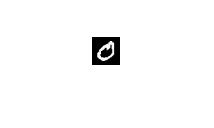
\includegraphics{/home/user/InFoMM/YearOne/WeekTwo/ImageClassificationTask/OpenImages/zero.jpg}
\includegraphics{/home/user/InFoMM/YearOne/WeekTwo/ImageClassificationTask/OpenImages/7.jpg}\includegraphics{/home/user/InFoMM/YearOne/WeekTwo/ImageClassificationTask/OpenImages/9.jpg}
%\end{figure}

The MNIST data stores each image as a 1-d column vector, with each row corresponding to a pixel. images from MNIST are stored vectors of length 784 (corresponding to an image of size 28x28pix). 

The basic principle then is to compare of each image in the test data against the images in the training data set, and find a way to match in order to classify according to the digit they most ressemble.   

Matlab will not open binary files. In order to access them therefore,  a simple way is to use the \texttt{loadMNISTImages.m} and \texttt{loadMNISTLabels.m}both available from\cite{load}.

\texttt{StartHere} provides the appriopriate, slightly modified, code for open images.

\section{Intensity.m - using the knn-algorithm}
The knn algorithm is a way of comparing a sample set against a wider data set. For a given a data set (in our case the column vector corresponding to the test image), it identifies the closest values (default metric is Euclidean) from within the training set.

It is important to understand the effect of choosing the appropriate value for \(k\). If the identified neighbours all have the same label, our confidence in the allocated label is greater. However, past a certain point, the chance of identifying incorrect labels increases, as matched images become further away from the test image.

Fig \ref{fig:IntensityMethod} illustrates effect of error of increasing \(k\) for the classification of 5000 images. The optimal value was found in this case to be k=4.

\begin{figure}[ht]
  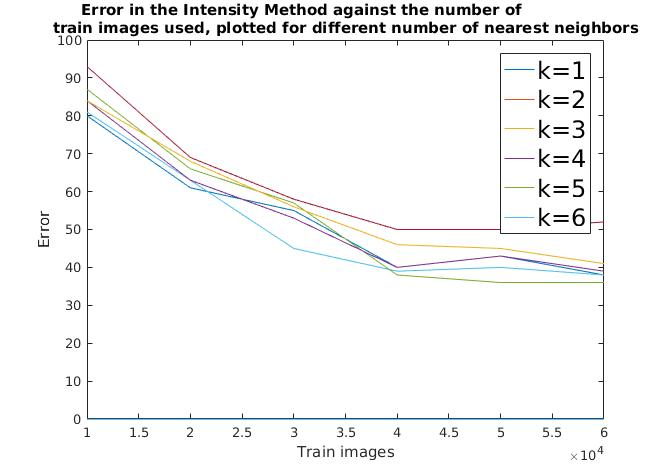
\includegraphics[width=\linewidth]{/home/user/InFoMM/YearOne/WeekTwo/ImageClassificationTask/Documentation/IntensityMethod.jpg}
  %\caption{The clusters generated by kmeans for 5000 images. Here, most of the clusters only have one or two digits represented, but some have as many as five, suggesting kmeans needs refining to make it more accurate.}
  \label{fig:IntensityMethod}
\end{figure}

\section{Intensity.m - Applying the method}

\texttt{Intensity.m} runs the knnmeans algorithm on the unaltered matrix, taking as input \(n\), the number of test images to use, \(p\), the number of training images to use, \(k\), the number of nearest neighbours to search. It provides as output, a vector \(a\) of length \(n\) composed of the recognised digits of the test images. 

It is important to note that  this method takes a lot of processing time, and some users may struggle to run the entire test image set (10000 images). 

A simple way to reduce the time taken for matching is to reduce the number of training images against which the test images are matched. \texttt{Intensityerror.m} has the same input as Intensity.m and returns the proportion of images which are wrongly classifed (ie, where the labels do not match their recognised values). It is worth noting that the error is largely unchanged whether we include 40,000 training images or the full 60,000.

However, by manipulating the data from the test images, we are able to reduce the time taken to run even further, without reducing the number of training images to compare against. This is because lots of information contained in the vector is irrelevant to its final class (eg. lighting conditions, discrepancies in the orientation of the shape).

\section{pcaerror.m - Reducing the number of feature vectors}

Principal component analysis is a way of identifying key features within a matrix. The process transforms the data to a coordinate system where the greatest variation lies on on the first co-ordinate (\emph{first principal components}). These components are also referred to as \emph{feature vectors} as the describe key features of the data. For a comprehensive review of the method, see \cite{pca}.

The function \texttt{pcaerror.m} performs principal component analysis on the test iamges and selects only the largest feature vectors, thereby reducing computation time. The function takes the same input as Intensity.m, with the addition of \(m\) which specifies the number of feature vectors.

Another alteration is to discard the first few feature vectors as well, as these will correspond to generic features of the whole data set (eg. lighting conditions). Within the code, this can be done by specifying the option\emph{d} as the number of early vectors to neglect. Note that any gains from doing this will be lost if \emph{d} is too large. Generally a value of 2 or 3 will achieve an increase in acccuracy and a decrease in cost. 

Fig \ref{fig:errorfeat} illustrates the effect of increasing the number of feature vector on decreasing the error. In this case, 20 feature vectors are enough to achieve a high degree of accuracy, whilst significantly reducing the cost. 

\begin{figure}
  \includegraphics[width=\linewidth]{/home/user/KiradjievKrisBeckerlegMel/pca.jpg}
  \caption{The effect of reducing the number of feature vectors following pca.}
  \label{fig:errorfeat}
\end{figure}

\section{Intensitymetric.m - Changing the metric}

Another aspect to consider is how distance between images should be measured. This is because Euclidean distance is not always best fitted to identify when images are very similar but have been altered through, for example have been rotated or translated.

\texttt{Intensitymetric.m} has the additional input of specifying a metric. this must be done as a string; ie: the spearman norm, \emph{'spearman'}, which considers the rank Spearman's coefficient between vectors, the cosine norm, \emph{'cosine'}, which considers one minus the interior angle between points, and the correlation norm, \emph{'correlation'}, which considers one minus the sample correlation between points. These three metrics all show decresase in the error and time taken, most notably with the correlation norm.

\section{Unsupervised case}

\begin{figure}[ht]
  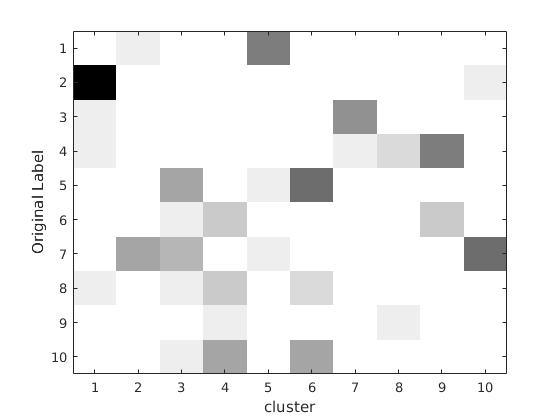
\includegraphics[width=\linewidth]{/home/user/InFoMM/YearOne/WeekTwo/ImageClassificationTask/clustering/kmeanscluster5000.jpg}
  \caption{The clusters generated by kmeans for 5000 images. Here, most of the clusters only have one or two digits represented, but some have as many as five, suggesting kmeans needs refining to make it more accurate.}
  \label{fig:cluster}
\end{figure}

The knn algorithm relies on a large sample of training data with which to compare images. Not only is this costly, it is not always possible to build such a set, and hence it is interesting to consider how unsupervised learning might be used instead.

\texttt{kmeanserror.m} looks at applying the kmeans algorithm to a sample of test data to sort it. This algorithm works by intialising a set of 'cluster means', assigning each data point to its nearest cluster mean, and then recursively recalculating the mean of all the elements in the cluster and reassigning elements to their new closest mean. Note that since we know the number of classes must correspond to the number of digits, we do not have any difficulty using a cluster method which requires knowing the number of clusters in advance. 

The function has for input \(n\), the number of images to test, and returns the proportion wrongly classified, as well as a pictorial representation of how text images were assigned.



The method has a quite high error relative to the supervised method, and different digits were frequently sorted into the same cluster, (see \ref{fig:cluster}). In order to improve the accuracy of the method, the vectors need to be treated such that the differences between those of different classes are emphasised and those within classes are downplayed. Methods similar to those outlined above for the training data approach may be useful in pursuing this further.

\section{Example}

The following code applies different methods to test 1000 images from the full 5000 images.

\insertcode{"/home/user/KiradjievKrisBeckerlegMel/Example.m"}{Find error and processing times for different methods.} 

% The first argument is the script location/filename and the second is a caption for the listing

\begin{thebibliography}{9}
\bibitem{MNIST}
Yann, LeCun. The MNIST Database [ONLINE] Available from \url{http://yann.lecun.com/exdb/mnist/}
\bibitem{load}
\emph{Using the MNIST Database} [ONLINE] Available from \url{http://ufldl.stanford.edu/wiki/index.php/Using_the_MNIST_Dataset}
\bibitem{pca}
\emph{Principal Component Analysis} [ONLINE] Available from \url{http://faculty.iiit.ac.in/~mkrishna/PrincipalComponents.pdf}
\end{thebibliography}

\end{document}

